 \documentclass[12pt]{article}
\usepackage[a4paper,  total={170mm,257mm},
 left=7mm,
 right=7mm,
 top=5mm,
 bottom=17mm
]{geometry}

\usepackage{array}
\usepackage{graphicx, subfig, wrapfig, fancyhdr, lastpage,makecell }
\newcommand\headerMe[2]{\noindent{}#1\hfill#2}
\usepackage[mathscr]{euscript}



\pagestyle{fancy}
\fancyhf{}

\cfoot{\em{Page \thepage \hspace{1pt} / \pageref{LastPage}}}
\begin{document}

\headerMe{Royaume du Maroc}{année scolaire \emph{2022-2023}}\\
\headerMe{Ministère de l'Éducation nationale, }{  Professeur :\emph{Zakaria Haouzan}}\\
\headerMe{du Préscolaire et des Sports}{Établissement : \emph{Lycée SKHOR qualifiant}}\\

\begin{center}

    \vspace{-1.5cm}
Devoir  N°4 - S1 \\
   Filière Tronc Commun Scientifique\\
Durée 3h00
\\
\hrulefill
\Large{Chimie 7pts - 63min}
\hrulefill\\

    \emph{Les  parties sont indépendantes}
\end{center}
%end Headerss------------------------
 
    \vspace{-1.2cm}
    
\section*{Partie 1 :La chimie autours de nous \dotfill (3pts) }
	
\textbf{1. }Compléter le tableau suivant:\dotfill(0,5pts)
\begin{center}
\begin{tabular}{ | c | c | c | }
	\hline
	\textbf{Espèce chimique }& \textbf{test} & \textbf{résultat} \\\hline 
 Présence d’eau $H_2O$ & Sulfate de cuivre anhydre & ....................... \\\hline  
 acide & ............. & ........................\\\hline 
\end{tabular}
\end{center}

\hspace{0.5cm}Depuis plus d’un siècle, l’eugénol est utilisée dans la médecine pour calmer la douleur des dents et la fièvre. 

\begin{wrapfigure}[10]{r}{0.32\textwidth}
	\vspace{-1.4cm}
	\begin{center}
    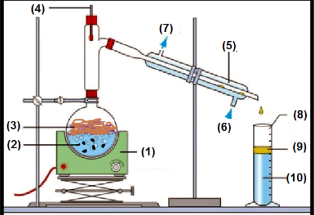
\includegraphics[width=0.32\textwidth]{./img/hydro.png}
	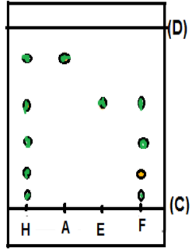
\includegraphics[width=0.2\textwidth]{./img/CCM.png}
\end{center}
\end{wrapfigure}

Dans cette partie, on s’intéresse à extraire l’eugénol du clou de
girofle, qui sont des boutons floral séché et contient une grande quantité de d’huile
essentielle trés riche en eugénol et d’acétyle eugénol.
\begin{enumerate}
	\item[I] \underline{\textbf{Première étape : l’extraction de l’eugénol.}}
		\begin{enumerate}
			\item[1.] Pour extraire l’huile essentielle des clous de girofle, on
introduit dans un ballon 100 ml d’eau distillée, 5g de clous de
girofle en poudre et quelques pierres ponce. Le ballon est placé dans
le montage suivant ci-contre.et on recueillit le distillat dans une
éprouvette graduée.
	\item[1.1.] donner le nom de ce montage, et donner son principe. \dotfill(0,5pts)

		\end{enumerate}
	\item[II] \underline{\textbf{Deuxième étape :séparation de deux phases. }}
		\begin{enumerate}
			\item [2.]On transvase le contenu de l’erlenmeyer dans une ampoule à \\décanter. On ajoute 10mL d’ un solvant
convenable pour la \\décantation. On agite le contenu de l’ampoule rigoureusement puis,\\ on enlève le bouchon
de l’ampoule et on laisse décanter son contenu.

Le tableau ci-dessous donne quelques propriétés des solvants :
\begin{center}
\begin{tabular}{ | c | c | c | c | }
	\hline
							& Cyclohexane & dichlométhane &éthanol  \\\hline 
	Densité				    & 0,89        & 1,34          & 0,78\\\hline  
	Miscililité avec l’eau  & Non miscible& Non miscible  & miscible\\\hline  
	Solubilité de l’eugénol & Peu soluble & Très soluble & Très soluble\\\hline  
\end{tabular}
\end{center}

\item[2.1]Dessiner sur votre copie l’ampoule à décanter et donner les noms des deux phases.puis choisir le solvant convenable pour cette extraction. Justifier.\dotfill(0,5pts)

		\end{enumerate}
		%\vspace{3cm}	
	\item[II] \underline{\textbf{Troisième étape : identification de l’espèce extraite.}}

%\begin{wrapfigure}[5]{r}{0.36\textwidth}
    %\vspace{-1.8cm}
    %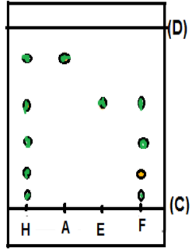
\includegraphics[width=0.36\textwidth]{./img/CCM.png}
%\end{wrapfigure}


		\begin{enumerate}
			\item[3].On réalise une chromathgraphie sur couche mince de l’huile essentielle extraite des clous de girofle. On
dépose quatre gouttes sur la plaque chromatographique.\\\textbf{(H):}L’huile essentielle extraite des clous de girofle. ; 
\\\textbf{(E):}Eugenol commercial. ; \textbf{(A:)}L’acétyle eugénol.
\\\textbf{(F:)}L’huile essentielle préparé à partir de feuilles de giroflier.
Après révélation on a obtenu le chromatogramme ci-contre.

\item[3.1.]Est-ce que l’huile essentielle (H) extraite des girofle est pure, justifier.\dotfill(0,5pts)
\item[3.2.]Quelles sont les espèces présentes dans cette huile essentielle (H) extraite des clous de girofle?\dotfill(0,5pts)

\item[3.3.]Calculer les rapports frontaux de l’eugenol commercial et de l’L’acétyle
eugénol.\dotfill(0,5pts) 
		\end{enumerate}
\end{enumerate}


\section*{Partie 2 :Constitution de la matière \dotfill (4pts) }
\begin{center}
\underline{\textbf{I. Le modèle de l'atome} }
\end{center}
L’atome de sodium Na contient 23 nucléons et 11 électrons.

Données : $m_p = m_n = 1,7.10^{-27}kg$ , $1pm = 10^{-12}m$ , $1m^3  =10^6 cm^3$

\begin{enumerate}
	\item[I.1.]  Donner la formule électronique de cet
atome .la couche externe est-elle saturée
justifier votre réponse.\dotfill(0,5pts)

\item[I.2.] Calculer le nombre des atomes de sodium
contenus dans un échantillon de sodium
de masse $m=23,20g$.\dotfill(0,5pts)
\item[I.3.]  Le rayon de l’atome de sodium est
$r=190pm$, calculer son volume exprimé en $m^3$ et $cm^3$.\dotfill(0,5pts)
\end{enumerate}

\begin{center}
\underline{\textbf{II. Géométrie de quelques molécules} }
\end{center}
%\begin{wrapfigure}[5]{r}{0.36\textwidth}
    %\vspace{-1.8cm}
    %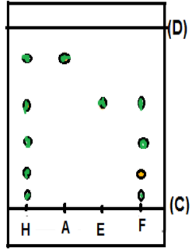
\includegraphics[width=0.36\textwidth]{./img/CCM.png}
%\end{wrapfigure}

On considère la molécule suivante de Chlorométhane $CH_3Cl$

\begin{enumerate}

	\item[II.1. ] Donner la structure électronique de carbone $C (Z=6)$, d’hydrogène $H (Z=1)$, et de chlore $Cl (Z=17)$ \dotfill(0,5pts)
	\item[II.2.]  Donner le nombre $n_t$ des électrons de la couche externe de chaque atome et Déterminer le nombre de doublets liants $n_l$ et non liants $n_{nl}$ pour chaque atome. \dotfill(0,5pts)

	\item[II.3.]  Représenter cette molécule selon le modèle de Lewis et déduire sa représentation de Cram \dotfill(0,5pts)

\end{enumerate}

\begin{center}
\underline{\textbf{III. Classification périodique des éléments chimiques } }
\end{center}

La couche électronique externe d'un atome est la couche (M). Elle comporte 1 électron. 
\begin{enumerate}

	\item[III.1.] Dans quelle période et quel groupe de la classification périodique appartient l'élément chimique correspondant ?\dotfill(0,5pts)
	\item[III.2] Nommer la famille à laquelle cet élément chimique appartient. Citer deux éléments appartenant à la
     même famille.  \dotfill(0.5pts)
\end{enumerate}




%__________________Chimie ______________________-
%%%%%%%+_+_+_+_+_+_+_+_+_Partie1

%_____________________________________PHYSIque Partie 22222____________________________________________________________________________
\begin{center}
    \vspace{0.5cm}
\hrulefill
\Large{Physique 13pts - 117min}
\hrulefill\\
	\emph{Les parties sont indépendantes}
\end{center}
%end Headerss------------------------

 \section*{Partie 1 :Interactions mécaniques \dotfill(4 pts)}

\begin{center}
			\underline{\textbf{I. la Gravitation universelle } }
\end{center}
 
Soient deux corps ponctuels A et B de masses respectives $m_A = 10Kg$ et $m_B=20Kg$
distants de:$d =10m$.

\begin{enumerate}

	\item[I.1] Donner les caractéristiques des deux forces de gravitation universelles               $\vec{F_{A/B}}$ et $\vec{F_{B/A}}$\dotfill(0,25pts)
	\item[I.2] Représenter sur le schéma ci-contre les  $\vec{F_{A/B}}$ et $\vec{F_{B/A}}$ en utilisant une échelle adapté.\dotfill(0,25pts)
\item[II.3] A une altitude h de la surface de la terre, l’intensité de la pesanteur $g_0$ est donnée par la formule \\suivante :$g = G.\frac{M_T}{(R_T + h)^2}$.

\item[I.3.1] En déduire l’expression de l’intensité du champ de pesanteur
$g_0$ la surface de la terre $(h=0)$ en \\fonction de :G,$M_T$,$R_T$. \dotfill(0,5pts)

\item[I.3.2] Déduire la relation $g=g_0.\frac{R_T^2}{(R_T + h)^2}$.\dotfill(0,5pts)
\item[I.3.3] Montrer que lorsque $h = 2.R_T$ On a $P=\frac{P_0}{9}$.\dotfill(0,5pts)
 \end{enumerate}
	%\vspace{1cm}
\begin{center}
	\vspace{0.99cm}
			\underline{\textbf{II.Exemples d’actions mécaniques } }
\end{center}


\begin{wrapfigure}[2]{r}{0.25\textwidth}
	
	\vspace{-1.8cm}
	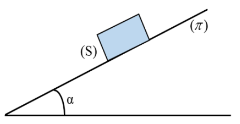
\includegraphics[width=0.25\textwidth]{./img/plan pi.png}
\end{wrapfigure}

Un corps solide (S) de masse m = 5kg est en équilibre sur un
plan incliné d’un angle $\alpha$ par rapport à l’horizontale.
\begin{enumerate}
	\item[II.1] Sachant que la force $\vec{R}$ exercée par le plan incliné sur le
		corps compense le poids $\vec{P}$ de ce corps.
		\begin{enumerate}
			\item Représenter sur le schéma de la figure la force l’échelle $1cm \rightarrow 20N$.\dotfill(0,5pts)
			\item Le contact entre le corps (S) et le plan incliné est-il avec ou sans frottement? justifier.\dotfill(0,5pts)

		\end{enumerate}
	\item[II.2] L’intensité de la force pressante $\vec{F}$ exercée sur la surface du plan incliné par le corps (S) représente
57.2\% du poids de ce dernier.
\begin{enumerate}
	\item Représenter la force $\vec{F}$ sur le schéma à la même échelle que précédemment.\dotfill(0,5pts)
	\item Déterminer la valeur de la pression $p$ à la surface du contact.avec l'aire du contact corps-plan incliné: $S = 40cm^2$\dotfill(0,5pts)
\end{enumerate}
\end{enumerate}


 \section*{Partie 2 :Le Mouvement rectiligne uniforme\dotfill(4 pts)}
\begin{wrapfigure}[4]{r}{0.3\textwidth}
	\begin{center}
		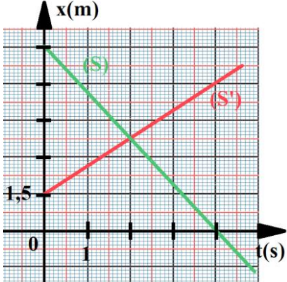
\includegraphics[width=0.3\textwidth]{./img/ex_Mvt.png}
	\end{center}
\end{wrapfigure}


	  Deux solides (S) et (S') ponctuels se déplacent sur l'axe (Ox) selon une
trajectoire rectiligne. Le graphe suivant représente la variation de x en
fonction du temps t de chaque solide.



\begin{enumerate}


	\item Retrouver $x_0$ la position du à l'origine des dates de chaque mobile.\dotfill(0,25pts)

	\item Donner la vitesse de chaque solide. Conclure.\dotfill(0,25pts)
	\item Donner la nature de déplacement du solide (S).\dotfill(0,25pts)
	\item Déterminer graphiquement la date quand les deux mobiles se
rencontrent-ils.\dotfill(0,25pts)
\item Donner x(t) et x'(t) les équations horaires du mouvement de chaque
mobile.\dotfill(0,25pts)
\item A l'aide des équations horaires du mouvement, vérifier la réponse de la question (4).\dotfill(0,25pts)

\end{enumerate}
\textbf{7. } On considère deux voitures A et B en mouvement rectiligne uniforme sur une partie d’une autoroute avec les vitesses respectivement $V_A=72Km.h^{-1}$ et $V_B=108Km.h^{-1}$.
%\begin{wrapfigure}{r}{0.36\textwidth}
	\vspace{-0.3cm}
 \begin{center}
	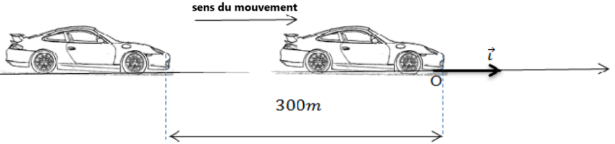
\includegraphics[width=0.56\textwidth]{./img/ex1.png}
\end{center}
%\end{wrapfigure}


	\vspace{-0.4cm}
A l’instant $t=0$ la voiture B est à $300m$ derrière la voiture A.
On choisit la position O, la position de la voiture A à l’instant $t=0$ ; comme origine des abscisses et des dates.


\begin{enumerate}
	\item[7.1]  Convertir la valeur de $V_A$ et $V_B$ en $m.s^{-1}$.\dotfill(0,5pts)
	\item[7.2]  Ecrire l’équation horaire du mouvement de chacune des voitures (A) et (B) sur l’axe $(Ox)$.\dotfill(1pt)
	\item[7.3]  Déterminer l’instant $t$ et l’abscisse $x$ du doublage de la voiture (A) par la voiture (B).\dotfill(1pt)
\end{enumerate}

 \section*{Partie 3 :Vérification du concept d'inertie.\dotfill(3 pts)}


\begin{wrapfigure}[4]{r}{0.36\textwidth}
	%\vspace{-0.8cm}
	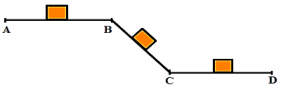
\includegraphics[width=0.36\textwidth]{./img/last.png}
\end{wrapfigure}


Un corps (S) se déplace sur un rail composé de 3 parties. On
lance ce corps du point A avec une vitesse $V_A=1m/s$ , et arrive au point D avec une vitesse $V_D=2m/s$. 

On considère que le contact se fait sans frottement.

\begin{enumerate}
	\item Faire l’inventaire des forces appliquées sur le corps (S), et représenter ces forces sur la figure pour
chaque partie. \dotfill(0,5pts)
\item Déterminer la partie où le principe d’inertie n’est pas vérifié.\dotfill(0,25pts)
\item Quelle est la valeur de la vitesse du corps (S) au point B, et au point C ? justifier votre réponse.\dotfill(0,25pts)
\end{enumerate}


\begin{wrapfigure}{r}{0.36\textwidth}
	\vspace{-0.8cm}
	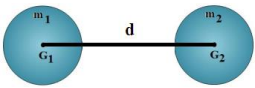
\includegraphics[width=0.36\textwidth]{./img/ex3.png}
\end{wrapfigure}

\begin{wrapfigure}[2]{r}{0.12\textwidth}
	\vspace{-3cm}
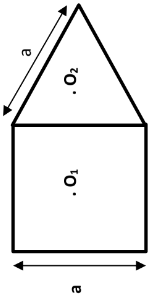
\includegraphics[width=0.12\textwidth]{./img/ex4.png}
\end{wrapfigure}

Deux sphères (A) et (B) de masses respectives $m_1$=$1kg$ et $m_2$=$3kg$ et de centres d’inertie respectives $G_1$ et $G_2$ qui sont séparés par la distance $d = 40 cm$. Ces deux sphères sont liées rigidement et constitue un système comme l’indique la figure ci-contre.

\begin{enumerate}

	\item[4.] Rappeler la relation barycentrique.\dotfill(0,25pts)
	\item[5.] Déterminer le centre d’inertie G de ce solide.\dotfill(0,25pt)
	\item[6.] Une plaque homogène et d’épaisseur constante, et formée d’une partie carrée et de côté $a=4cm$, et d’une partie triangulaire équilatérale.

	Sachant que \textbf{la masse} de la partie triangulaire est \textbf{3 fois plus légère} que la masse de la partie carrée.

	déterminer la position du centre de masse de la plaque homogène par application d’une méthode de votre choix.\dotfill(1,5pts)
\end{enumerate}

 \section*{Partie 4 :La poussée d'Archimède exercée sur un pavé \dotfill(2 pts)}
Un pavé flotte à la surface de l’eau. Ses dimensions sont : $h = 20 cm$ ,  $L = 60 cm$ ,  $l = 20 cm$.

\begin{wrapfigure}{r}{0.38\textwidth}
	\vspace{-4.3cm}

	
 \begin{center}
	 \hspace{-3cm}	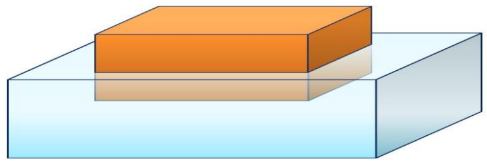
\includegraphics[width=0.38\textwidth]{./img/img01.png}
\end{center}
\end{wrapfigure}
\begin{enumerate}
	\item  Le pavé émerge sur une hauteur de $h' = 17 cm$. Calculer le volume V' de la partie immergée.\dotfill{0,25pts}

	\item  Calculer la masse $m'_{dep}$ d’eau déplacée.\dotfill{0,25pts}
	\item  Calculer le poids $P'_{dep}$ d’eau déplacé.\dotfill{0,25pts}
	\item  déduire la valeur du poids P du pavé.\dotfill{0,25pts}
	\item  Préciser le matériau constituant ce pavé.\dotfill{1pt}
\end{enumerate}

\textbf{Donnée: } La masse volumique d'eau: $\rho_{eau} = 1000 kg/m^3$ , L'intensité de pesanteur: $g = 10N/kg$.

\begin{center}
\begin{tabular}{ |c| c| c| c|c|c| }
	\hline
	\textbf{Matériau}                   & Polystyrène & Bois &glace &Aluminium&Fer\\\hline 
	\textbf{Masse volumique} $(kg/m^3)$ & 11 & 850 &920 &2700& 8000\\\hline
\end{tabular}
\end{center}













\end{document}
